\documentclass{article}
\usepackage[utf8]{inputenc}
\usepackage{polski}
\usepackage{geometry}
\usepackage{pdfpages}
\usepackage{pdfpages}
\usepackage{listings}
\usepackage{listingsutf8}
\usepackage{multirow}
\usepackage{siunitx}
\usepackage{multirow}
\usepackage{booktabs}
\usepackage{tabularx}
\usepackage{placeins}
\usepackage{pdflscape}
\usepackage{graphicx}
\usepackage{subfig}
\usepackage{hyperref}
\usepackage{amsmath}
\usepackage{colortbl}

\geometry{
a4paper,
total={170mm,257mm},
left=20mm,
top=20mm
}
\newcolumntype{Y}{>{\centering\arraybackslash}X}
% \renewcommand\thesection{}
\lstset{%
literate=%
 {ą}{{\k{a}}}1
 {ę}{{\k{e}}}1
 {Ą}{{\k{A}}}1
 {Ę}{{\k{E}}}1
 {ś}{{\'{s}}}1
 {Ś}{{\'{S}}}1
 {ź}{{\'{z}}}1
 {Ź}{{\'{Z}}}1
 {ń}{{\'{n}}}1
 {Ń}{{\'{N}}}1
 {ć}{{\'{c}}}1
 {Ć}{{\'{C}}}1
 {ó}{{\'{o}}}1
 {Ó}{{\'{O}}}1
 {ż}{{\.{z}}}1
 {Ż}{{\.{Z}}}1
 {ł}{{\l{}}}1
 {Ł}{{\l{}}}1
}

\title{Metody Programowania Równoległego\\ Raport II - OpenMP}
\author{Maciej Trątnowiecki}
\date{AGH, Semestr Letni, 2022}

\begin{document}
    \maketitle
    \lstset{ 
      backgroundcolor=\color{white},   % choose the background color; you must add \usepackage{color} or \usepackage{xcolor}; should come as last argument
      basicstyle=\footnotesize,        % the size of the fonts that are used for the code
      breakatwhitespace=false,         % sets if automatic breaks should only happen at whitespace
      breaklines=true,                 % sets automatic line breaking
      captionpos=b,                    % sets the caption-position to bottom
      commentstyle=\color{mygreen},    % comment style
      deletekeywords={...},            % if you want to delete keywords from the given language
      escapeinside={\%*}{*)},          % if you want to add LaTeX within your code
      %extendedchars=true,              % lets you use non-ASCII characters; for 8-bits encodings only, does not work with UTF-8
      firstnumber=1000,                % start line enumeration with line 1000
      frame=single,	                   % adds a frame around the code
      keepspaces=true,                 % keeps spaces in text, useful for keeping indentation of code (possibly needs columns=flexible)
      keywordstyle=\color{blue},       % keyword style
      language=Octave,                 % the language of the code
      morekeywords={*,...},            % if you want to add more keywords to the set
      numbers=left,                    % where to put the line-numbers; possible values are (none, left, right)
      numbersep=5pt,                   % how far the line-numbers are from the code
      numberstyle=\tiny\color{mygray}, % the style that is used for the line-numbers
      rulecolor=\color{black},         % if not set, the frame-color may be changed on line-breaks within not-black text (e.g. comments (green here))
      showspaces=false,                % show spaces everywhere adding particular underscores; it overrides 'showstringspaces'
      showstringspaces=false,          % underline spaces within strings only
      showtabs=false,                  % show tabs within strings adding particular underscores
      stepnumber=2,                    % the step between two line-numbers. If it's 1, each line will be numbered
      stringstyle=\color{mymauve},     % string literal style
      tabsize=2,	                   % sets default tabsize to 2 spaces
      title=\lstname                   % show the filename of files included with \lstinputlisting; also try caption instead of title
    }
    % \lstinputlisting[language=bash]{no_qos.txt}
        % \begin{center}
        %     \includegraphics[width=13cm]{lab2/report/ex3_1.png}
        % \end{center}\\
        
    \section{Implementacja równoległego generowania losowych danych wejściowych}
        \subsection{Definicja problemu}
        W ramach zadania przygotowaliśmy implementację programu generującego równolegle losowe dane wejściowe dla algorytmu sortującego. Implementacja przygotowana została w języku C, za wykorzystaniem interfejsu \textit{OpenMP}. Kod implementacji dla poszczególnych wersji programu załączono w ostatniej sekcji sprawozdania. \\
        Tak przygotowany program wykorzystaliśmy do pomiaru czasu wykonania i przyśpieszenia algorytmu, dla różnych ustawień klauzuli \textit{schedule}.
    
        \subsection{Pomiary i wyniki}
        Każdy z pomiarów powtórzyliśmy dziesięciokrotnie dla danych ustawień parametrów programu. Program testowaliśmy dla ustawień klauzuli \textit{schedule} ze zbioru \textit{guided}, \textit{dynamic} i \textit{static}, oraz wartości parametru \textit{chunk} z zakresu opisanego w tabeli poniżej.  
        
        \begin{center}
            \begin{table}[ht]
                \centering
                \begin{tabular}{|c|c|c|}
                    \hline
                    Schedule  & Chunk\\
                    \specialrule{1pt}{1pt}{1pt}
                    Dynamic & 1 \\
                    Dynamic & 1000\\
                    Dynamic & Rozmiar Problemu / Ilość CPU \\
                    Guided & 1\\
                    Static & Rozmiar Problemu / Ilość CPU \\
                    \hline
                \end{tabular}
                \caption{Parametry programu wykorzystane do przygotowania pomiarów.}
            \label{tab:my_label}
            \end{table}
        \end{center}
        Program uruchamialiśmy dla problemów o rozmiarze $10^6$, $10^7$ i $10^8$. Zebrane wyniki pomiarów czasu wykonania programu przedstawione zostały na poniższych wykresach.
        
        \newpage
        \begin{figure}[h!]
            \centering
            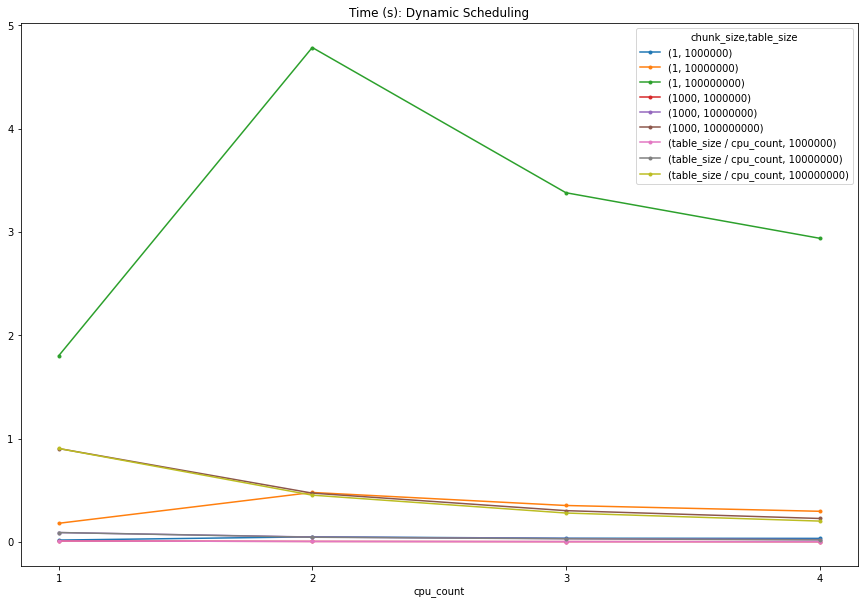
\includegraphics[width=17cm]{report2/images/Type/ex3_dynamic_mean.png}
            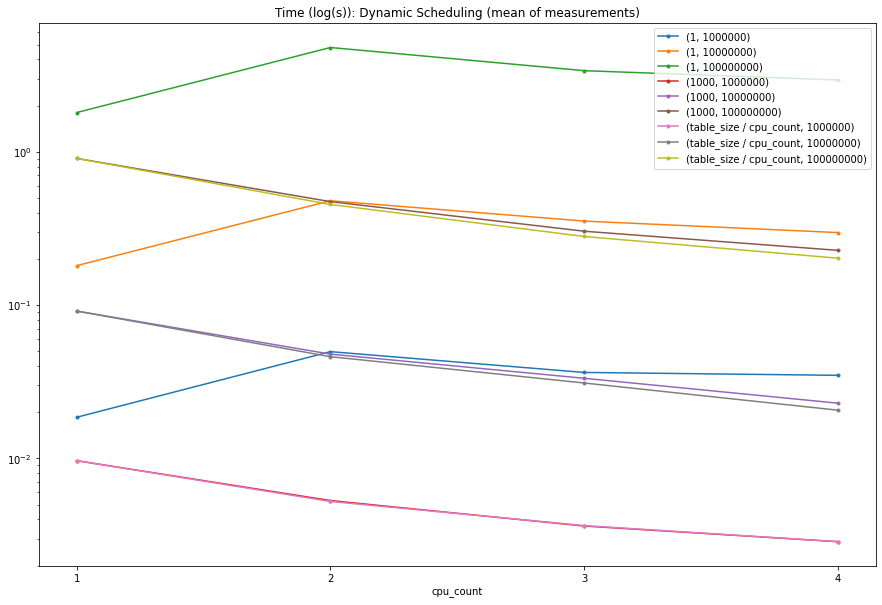
\includegraphics[width=17cm]{report2/images/Type/ex3_dynamic_mean_log.png}
            \caption{Pomiar czasu wykonania programu, Dynamic schedule, w zależności od parametrów. Uśrednione wartości z powtórzeń pomiarów. }
        \end{figure}
        \begin{figure}[h!]
            \centering
            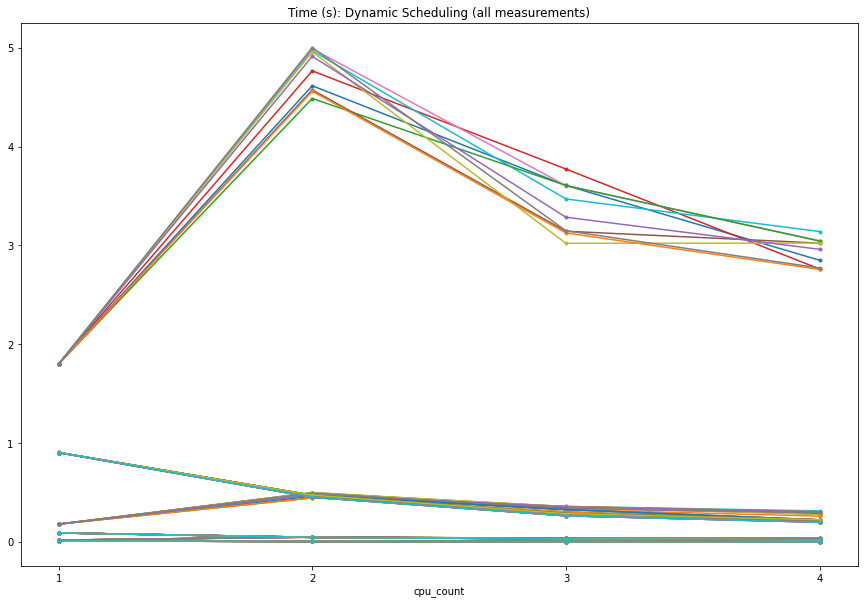
\includegraphics[width=17cm]{report2/images/Type/ex3_dynamic_all.png}
            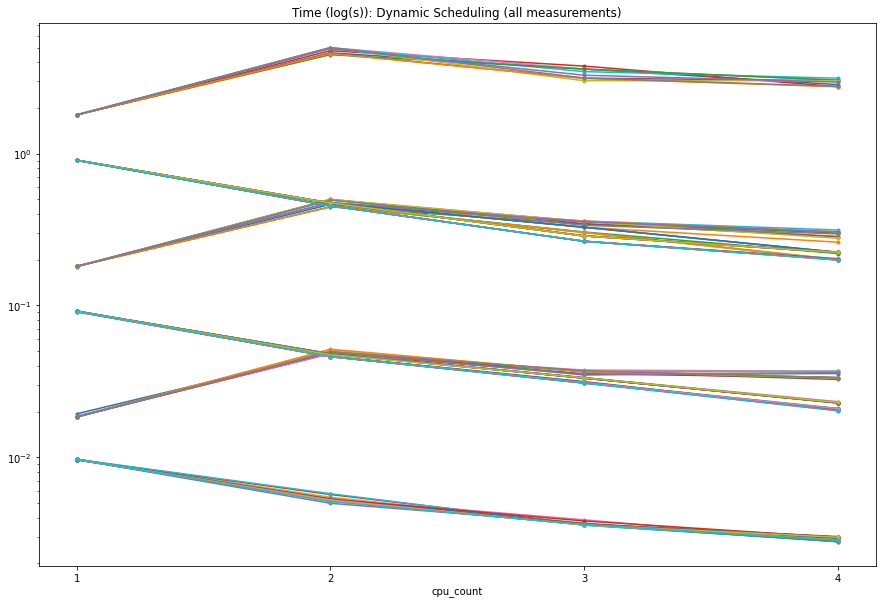
\includegraphics[width=17cm]{report2/images/Type/ex3_dynamic_all_log.png}
            \caption{Pomiar czasu wykonania programu, Dynamic schedule. Wszystkie pomiary. }
        \end{figure}
        \newpage
        \begin{figure}[h!]
            \centering
            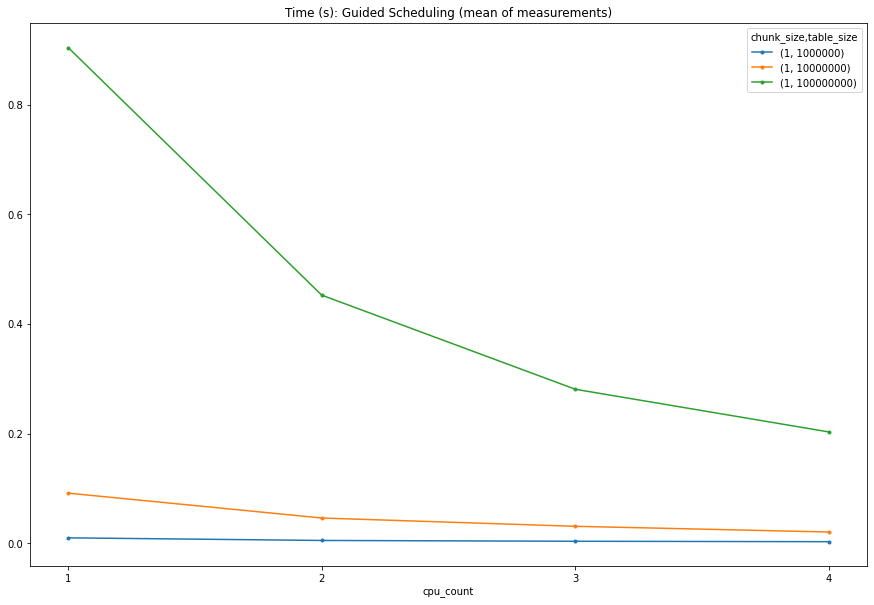
\includegraphics[width=17cm]{report2/images/Type/ex3_guided_mean.png}
            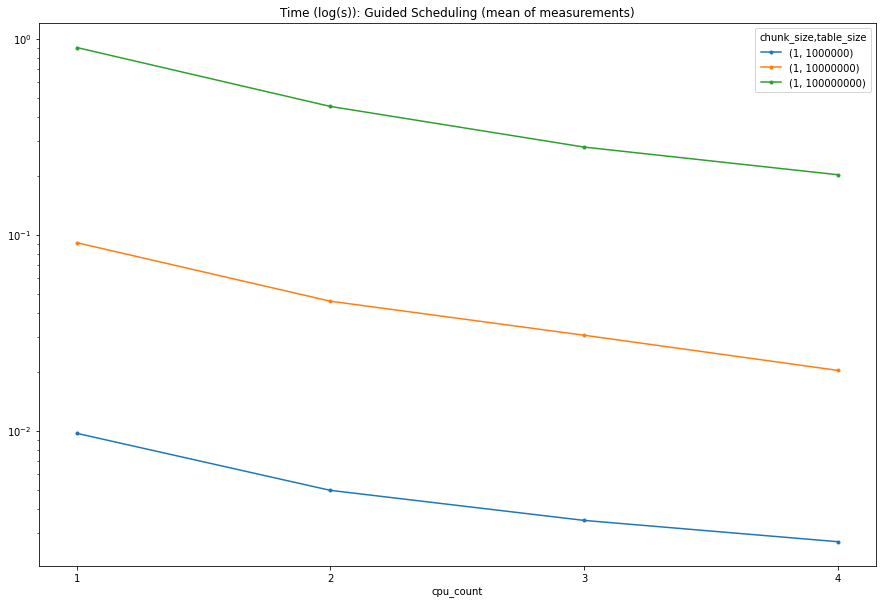
\includegraphics[width=17cm]{report2/images/Type/ex3_guided_mean_log.png}
            \caption{Pomiar czasu wykonania programu, guided schedule, w zależności od parametrów. Uśrednione wartości z powtórzeń pomiarów. }
        \end{figure}
        \newpage
        \begin{figure}[h!]
            \centering
            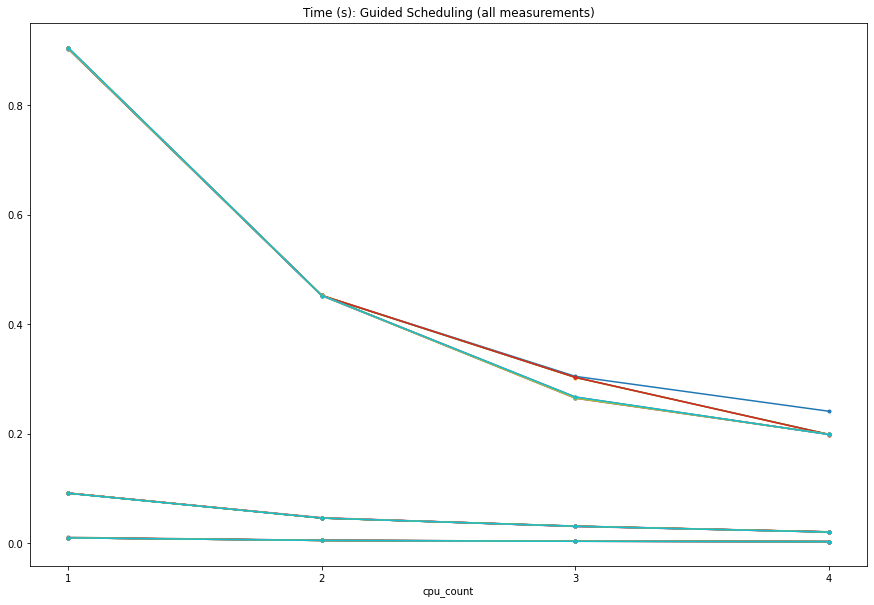
\includegraphics[width=17cm]{report2/images/Type/ex3_guided_all.png}
            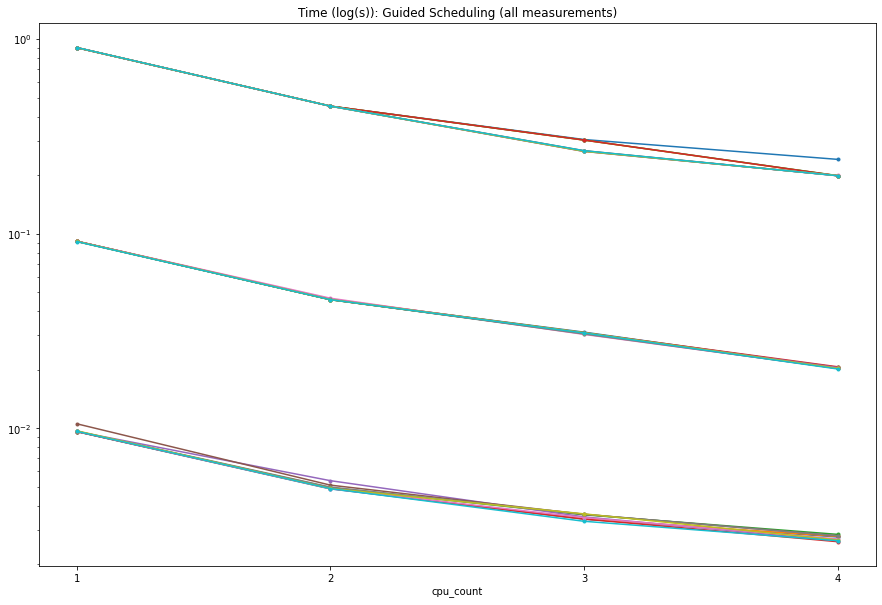
\includegraphics[width=17cm]{report2/images/Type/ex3_guided_all_log.png}
            \caption{Pomiar czasu wykonania programu, guided schedule. Wszystkie pomiary. }
        \end{figure}
        \newpage
        \begin{figure}[h!]
            \centering
            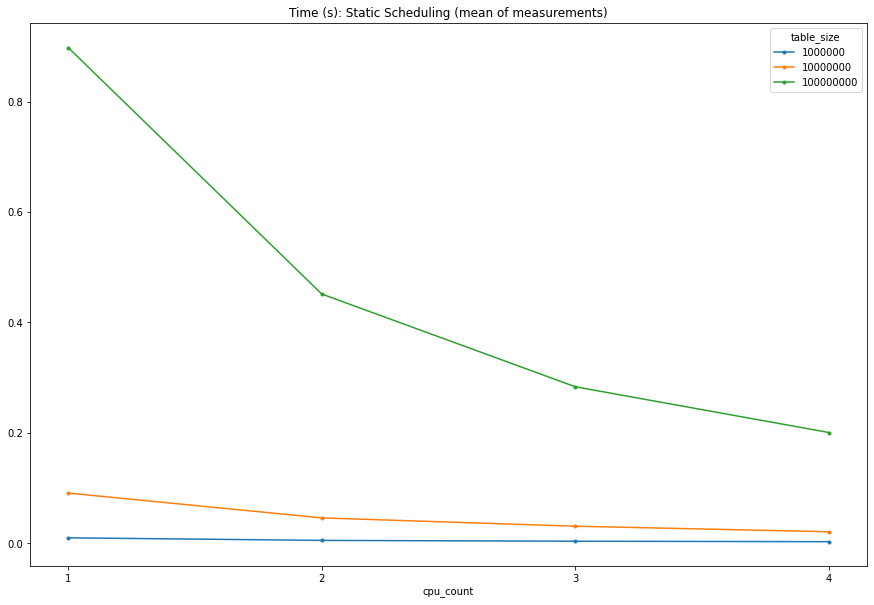
\includegraphics[width=17cm]{report2/images/Type/ex3_static_mean.png}
            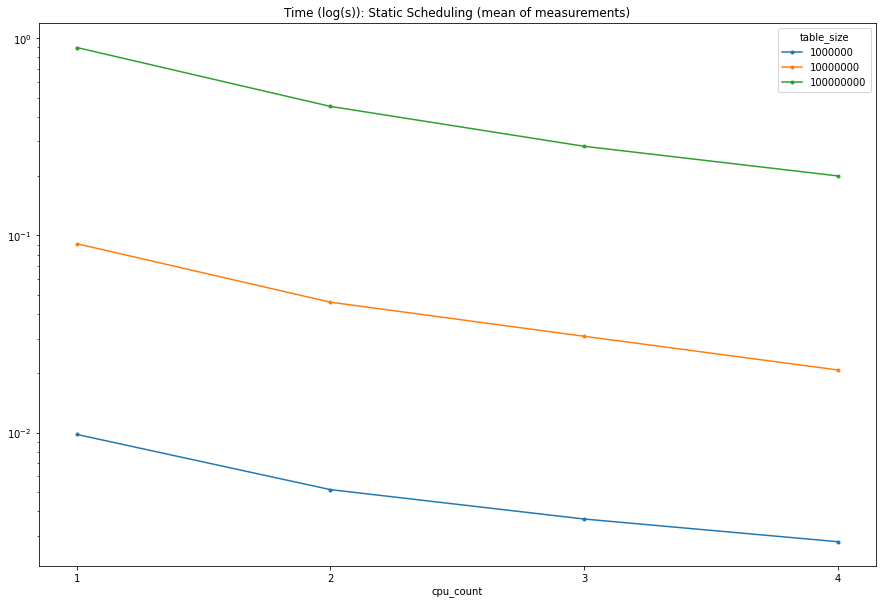
\includegraphics[width=17cm]{report2/images/Type/ex3_static_mean_log.png}
            \caption{Pomiar czasu wykonania programu, static schedule, w zależności od parametrów. Uśrednione wartości z powtórzeń pomiarów. }
        \end{figure}
        \newpage
        \begin{figure}[h!]
            \centering
            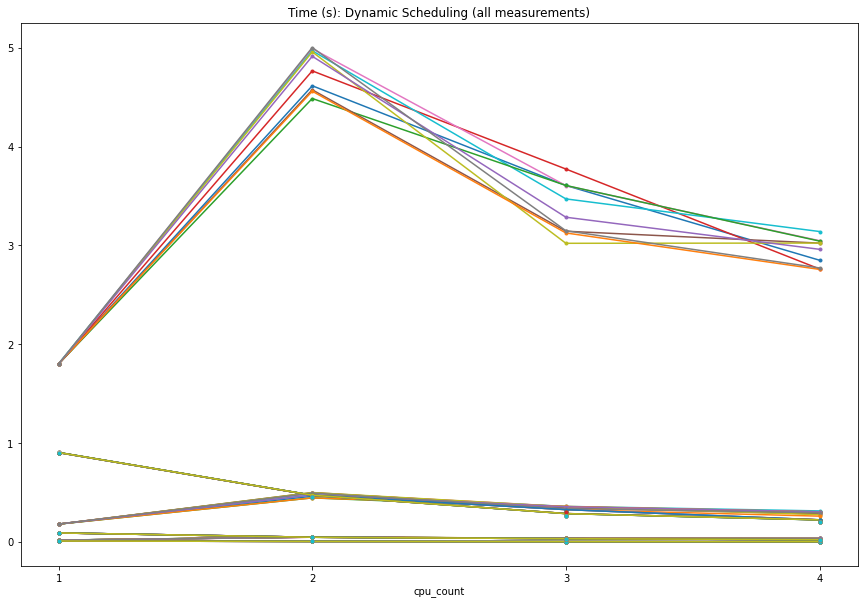
\includegraphics[width=17cm]{report2/images/Type/ex3_static_all.png}
            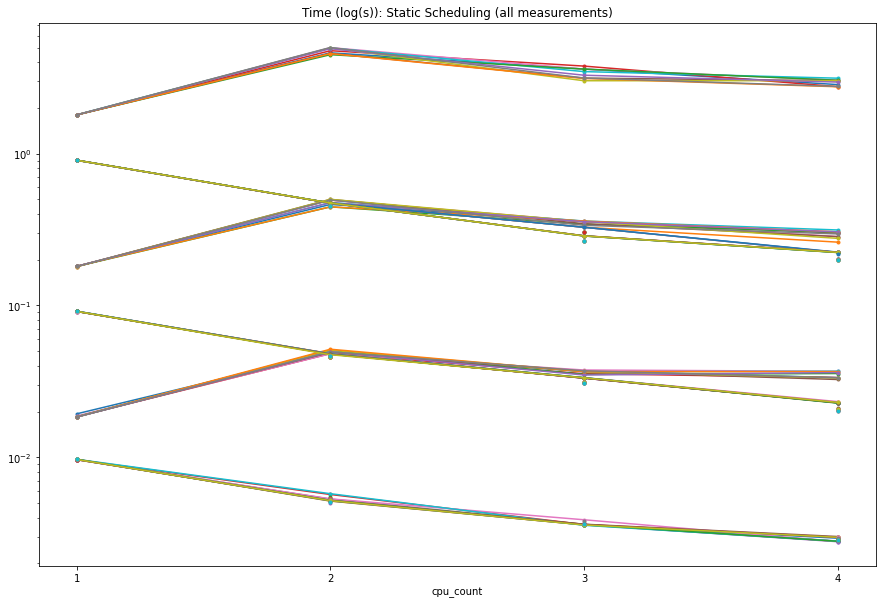
\includegraphics[width=17cm]{report2/images/Type/ex3_static_all_log.png}
            \caption{Pomiar czasu wykonania programu, static schedule. Wszystkie pomiary. }
        \end{figure}
        \newpage
        \begin{figure}[h!]
            \centering
            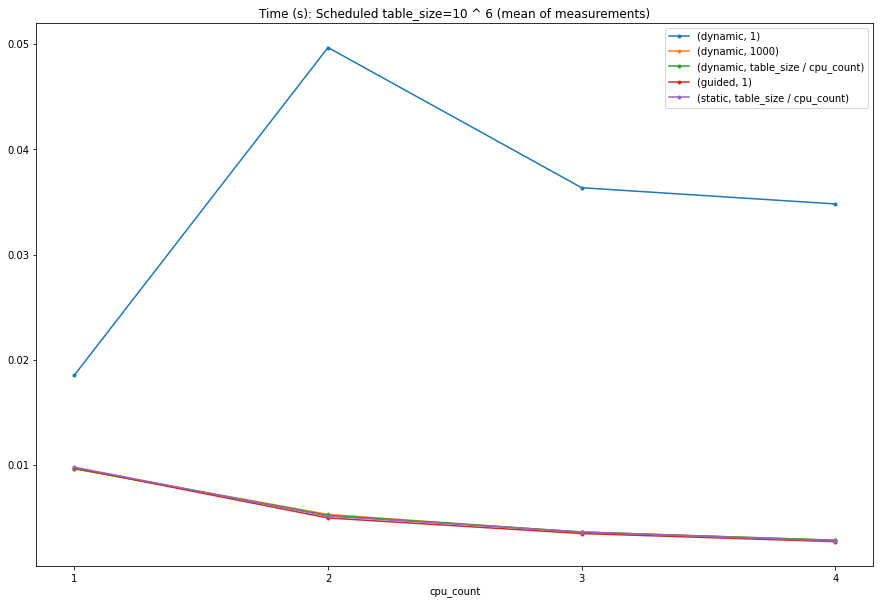
\includegraphics[width=17cm]{report2/images/TableSize/ex3_tb6_mean.png}
            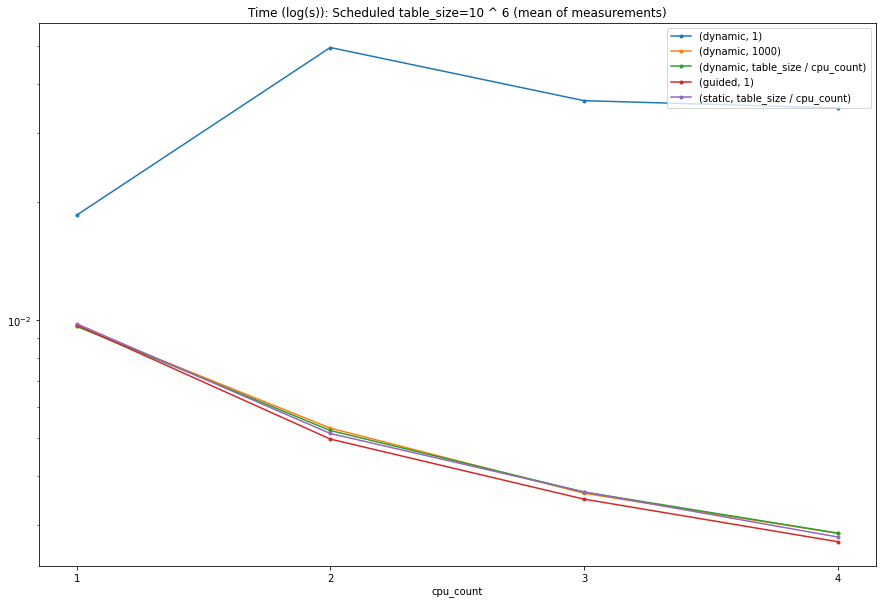
\includegraphics[width=17cm]{report2/images/TableSize/ex3_tb6_mean_log.png}
            \caption{Pomiar czasu wykonania programu, dla problemu rozmiaru 10 ** 6, w zależności od parametrów. Uśrednione wartości z powtórzeń pomiarów. }
        \end{figure}
        \newpage
        \begin{figure}[h!]
            \centering
            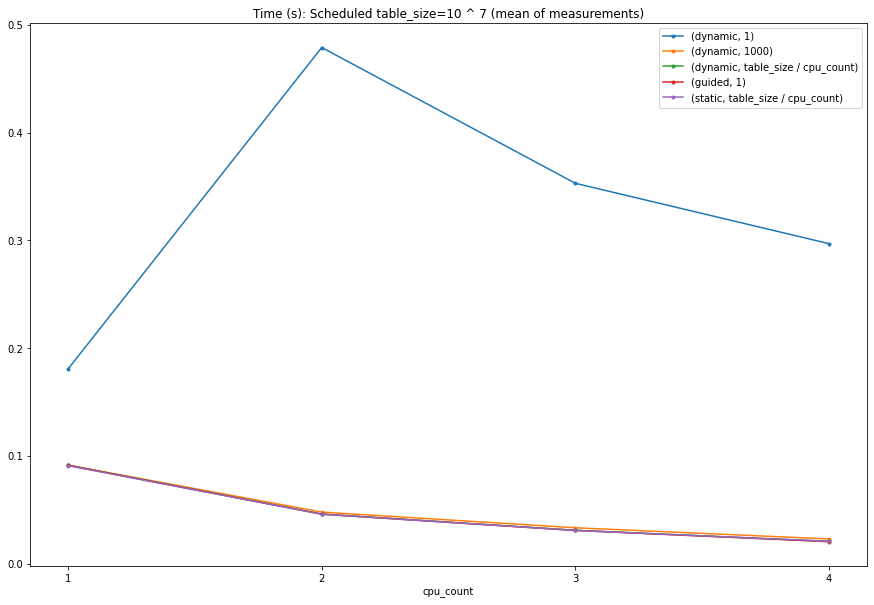
\includegraphics[width=17cm]{report2/images/TableSize/ex3_tb7_mean.png}
            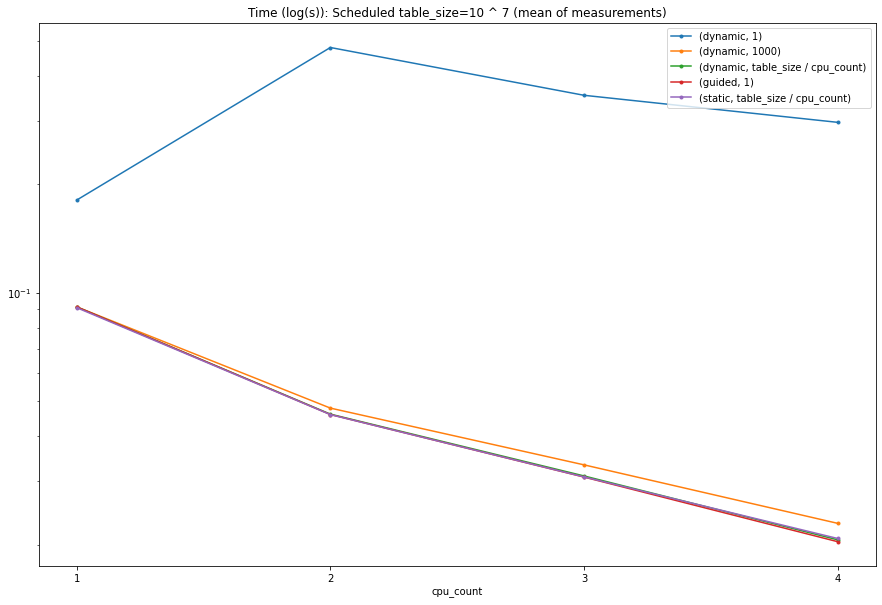
\includegraphics[width=17cm]{report2/images/TableSize/ex3_tb7_mean_log.png}
            \caption{Pomiar czasu wykonania programu, dla problemu rozmiaru 10 ** 7, w zależności od parametrów. Uśrednione wartości z powtórzeń pomiarów. }
        \end{figure}
        \newpage
        \begin{figure}[h!]
            \centering
            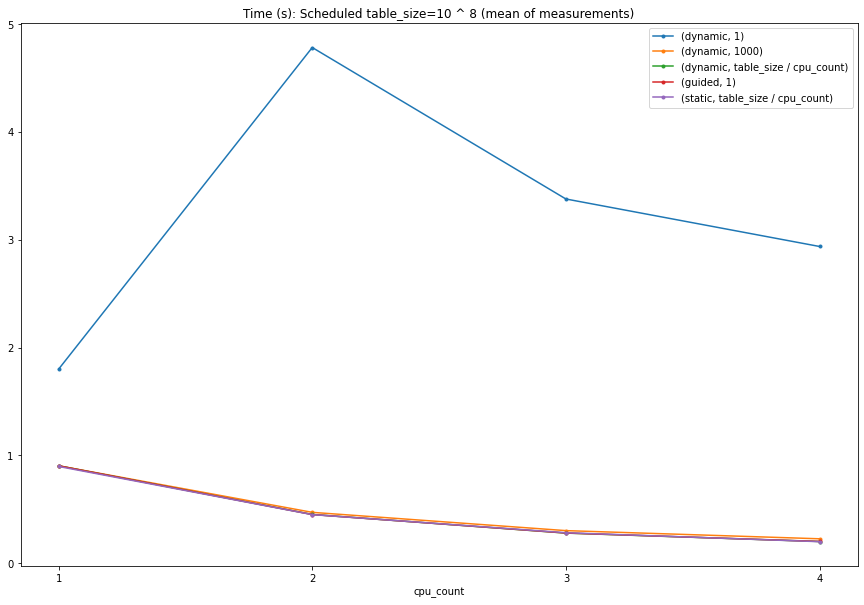
\includegraphics[width=17cm]{report2/images/TableSize/ex3_tb8_mean.png}
            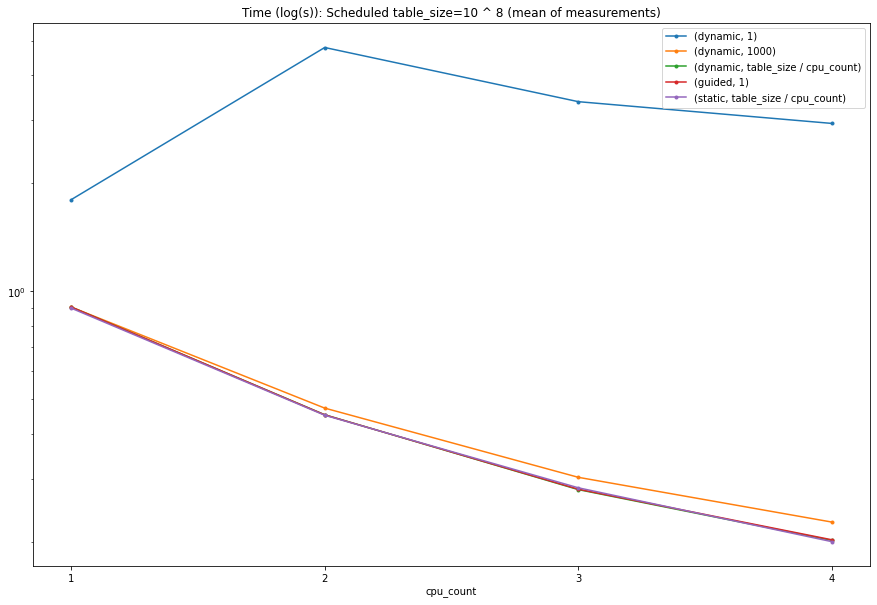
\includegraphics[width=17cm]{report2/images/TableSize/ex3_tb8_mean_log.png}
            \caption{Pomiar czasu wykonania programu, dla problemu rozmiaru 10 ** 8, w zależności od parametrów. Uśrednione wartości z powtórzeń pomiarów. }
        \end{figure}
        \newpage


        Na podstawie zmierzonych czasów pracy przygotowaliśmy także wykresy przyśpieszenia programu.
        \begin{figure}[h!]
            \centering
            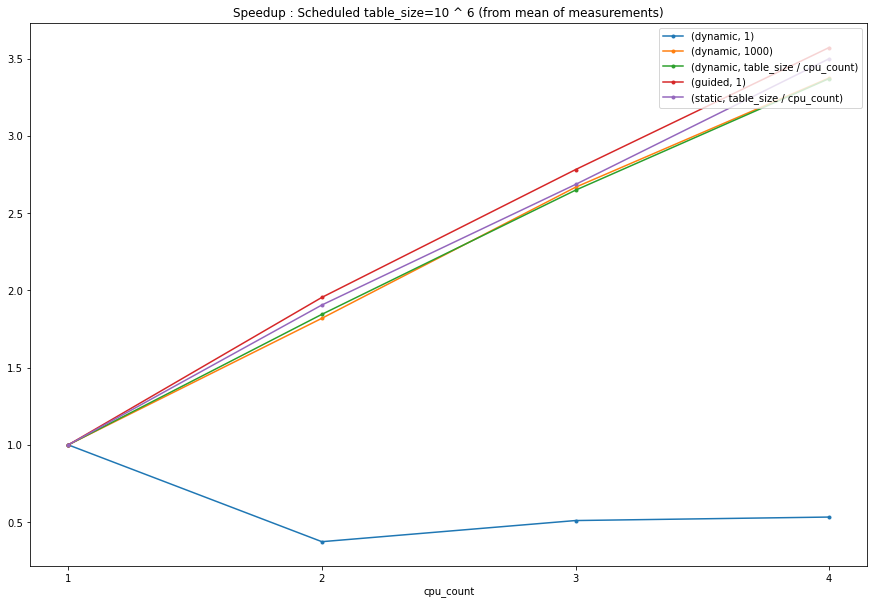
\includegraphics[width=17cm]{report2/images/TableSize/ex3_tb6_speedup.png}
            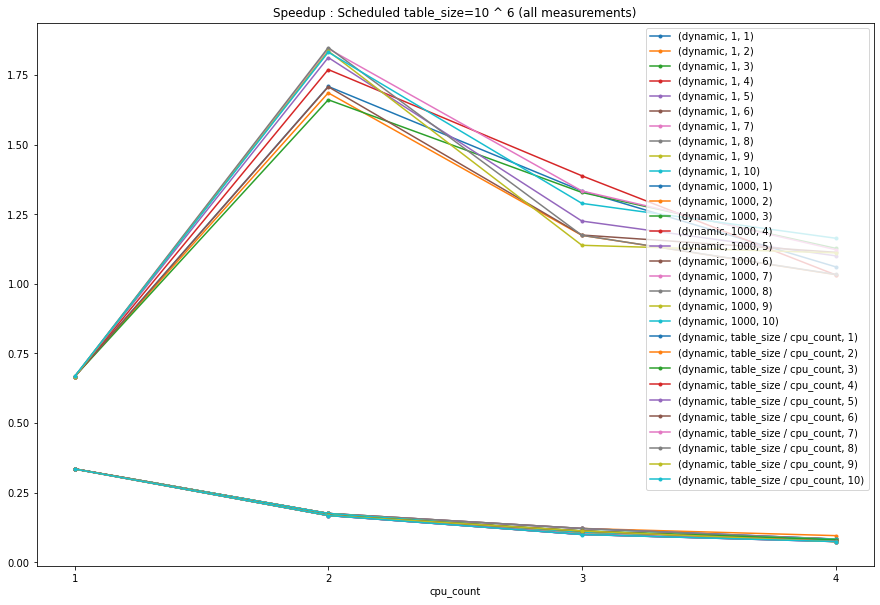
\includegraphics[width=17cm]{report2/images/TableSize/ex3_tb6_speedup_all.png}
            \caption{Pomiar przyśpieszenia czasu wykonania programu, dla problemu rozmiaru 10 ** 6, w zależności od parametrów. Uśrednione wartości z powtórzeń pomiarów. }
        \end{figure}
        \newpage
        \begin{figure}[h!]
            \centering
            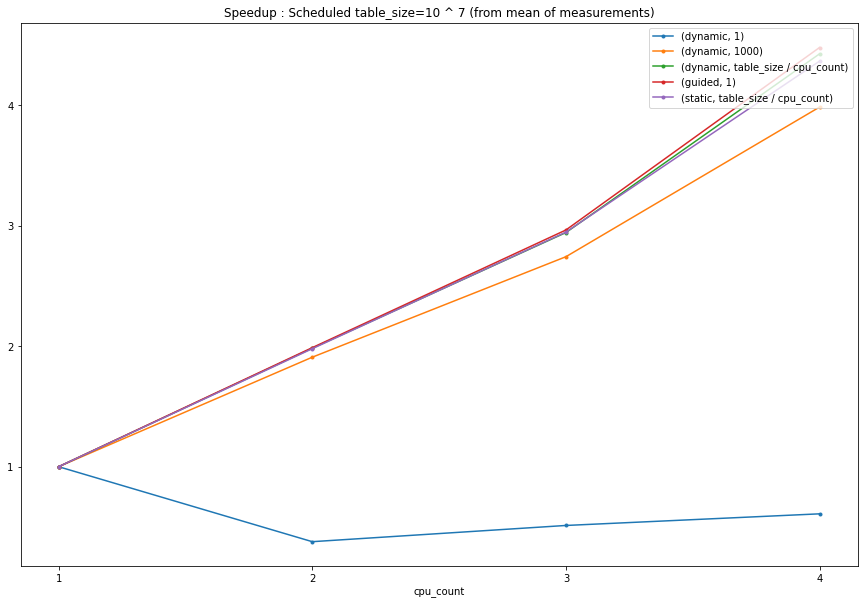
\includegraphics[width=17cm]{report2/images/TableSize/ex3_tb7_speedup.png}
            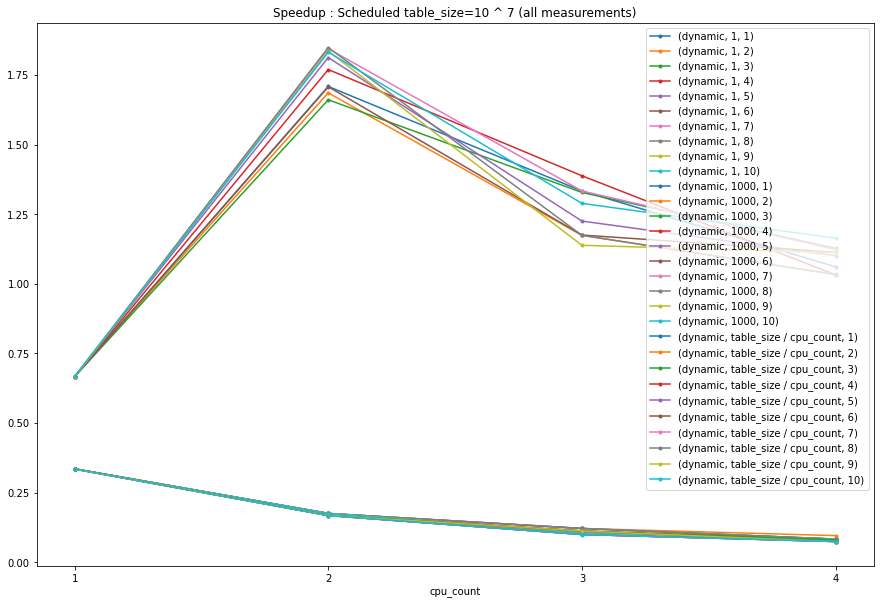
\includegraphics[width=17cm]{report2/images/TableSize/ex3_tb7_speedup_all.png}
            \caption{Pomiar przyśpieszenia czasu wykonania programu, dla problemu rozmiaru 10 ** 7, w zależności od parametrów. Uśrednione wartości z powtórzeń pomiarów. }
        \end{figure}
        \newpage
        \begin{figure}[h!]
            \centering
            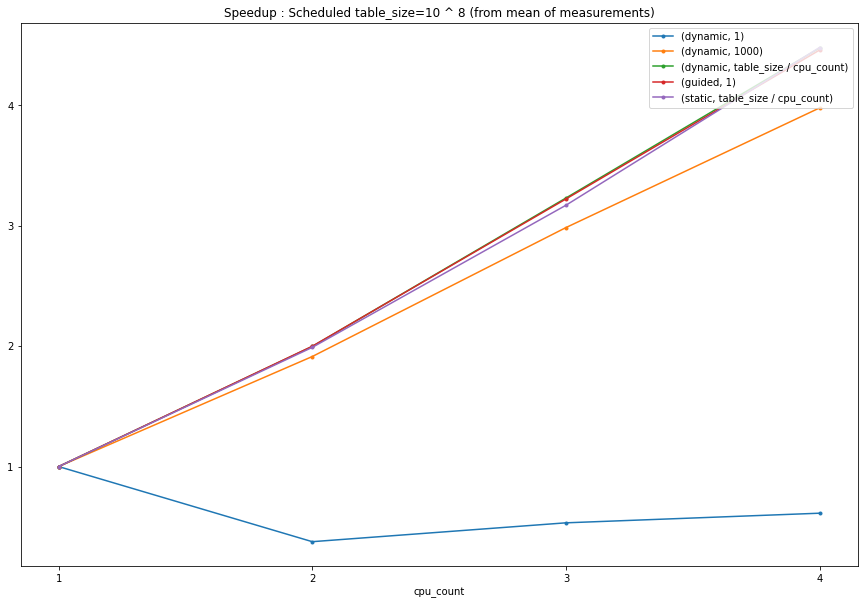
\includegraphics[width=17cm]{report2/images/TableSize/ex3_tb8_speedup.png}
            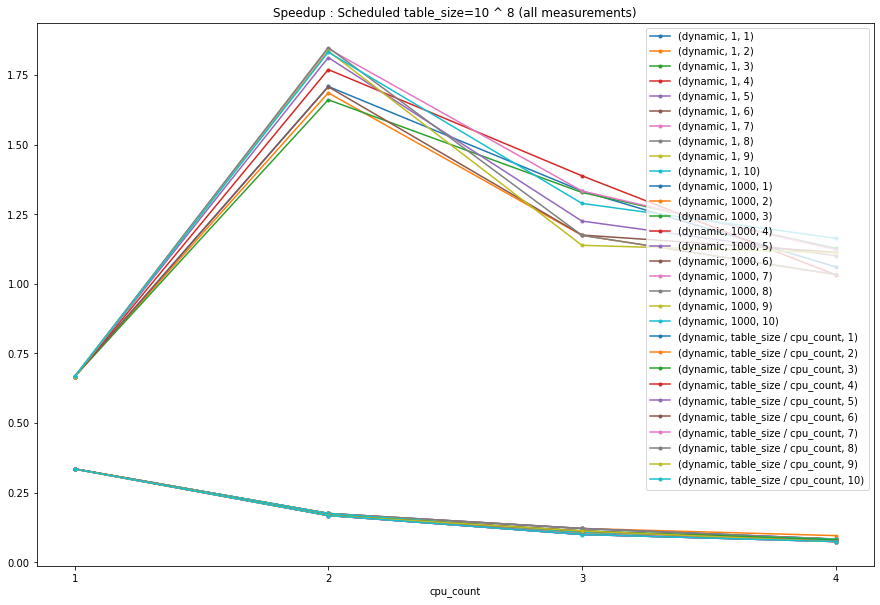
\includegraphics[width=17cm]{report2/images/TableSize/ex3_tb8_speedup_all.png}
            \caption{Pomiar przyśpieszenia czasu wykonania programu, dla problemu rozmiaru 10 ** 8, w zależności od parametrów. Uśrednione wartości z powtórzeń pomiarów. }
        \end{figure}


        \newpage
        \subsection{Badanie rozkładu uzyskiwanych liczb pseudolosowych}
        \textbf{Badanie poprawności danych wejściowych wobec założeń sortowania kubełkowego.}\\
        W celu zbadania rozkładu otrzymywanych z generatora liczb pseudolosowych przygotowany został duży zbiór liczb zwracanych przez generator, o rozmiarze $100 000 000$. Uzyskane liczby zostały przedstawione na histogramie grupującym obserwacje w $100$ kubełkach.
        \begin{figure}[h!]
            \centering
            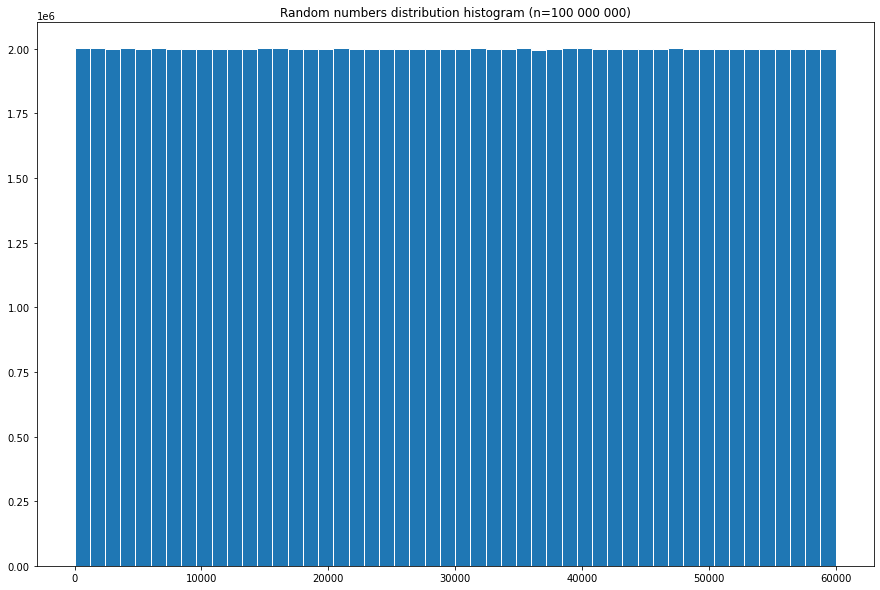
\includegraphics[width=17cm]{report2/images/RandomGen/random_dist_histo_100000000.png}
            \caption{Histogram przedstawiający rozkład uzyskiwanych z generatora liczb pseudolosowych. }
        \end{figure}
        
        Na podstawie histogramu wnioskować możemy, że otrzymywany rozkład z generatora jest równomierny. Tak przygotowany generator dobrze sprawdzi się podczas testowania algorytmów sortujących.

        \subsection{Wnioski}
        Analizując otrzymane wyniki pomiarów, zauważyć możemy że każda z typów klauzuli \textit{schedule} pozwoliła na uzyskanie zadowalających i porównywalnych przyśpieszeń, pod warunkiem wybrania odpowiedniej wartości parametru \textit{chunk}. W szczególności, klauzula \textit{guided} odpowiednio radzi sobie z jego dobraniem. Zauważyć możemy znaczny spadek wydajności, w przypadku wybrania zbyt małej wartości tego parametru dla wersji \textit{dynamic}, skutkującego nawet obniżeniem wydajności programu pomimo większej liczby dostępnych procesorów. 
        
        % \newpage
        \subsection{Kod programu}
        \lstinputlisting[language=c]{../ex3/schedule_static.c}
        \lstinputlisting[language=c]{../ex3/schedule_dynamic.c}
        \lstinputlisting[language=c]{../ex3/schedule_guided.c}
        
    \newpage 
    
    \section{Implementacja równoległego algorytmu sortowania kubełkowego}
    \subsection{Wstęp}
    W ramach ćwiczeń laboratoryjnych przygotowaliśmy wraz z kolegą z grupy implementację algorytmu sortowania kubełkowego w sposób równoległy dla tego samego sposobu generowania liczb pseudolosowych i struktury danych przechowujących kubełki na dwa różne sposoby. W implementacji kolegi każdy z wątków czytał całą tablicę wejściową i rozdzielał liczby do przypisanych do niego kubełków. W mojej implementacji, każdy z wątków czytał jedynie fragment tablicy i rozdzielał liczby do odpowiedniego kubełka (z synchronizacją na dostępie do kubełka, dostęp do tablicy nie musi być synchronizowany). Na potrzeby sprawozdania będę nazywał te implementacje odpowiednio wersją pierwszą i druga algorytmu. \\
    
    Testy i pomiary czasowe wykonania algorytmu wykonane zostały na procesorze \textit{Apple M1 Max} (chyba że wskazano inaczej) wykonanym w architekturze \textit{ARM} o $10$ rdzeniach roboczych, przy czym wskazać należy że procesor posiada $8$ rdzeni wysokiej wydajności i $2$ rdzenie energooszczędne co może zaburzać obserwowane wyniki przyśpieszenia.  \\
    Każdy z pomiarów wykonany został dziesięciokrotnie, a wyniki uśrednione. 
        
    \subsection{Struktura danych}
    W obu algorytmach do przechowywania kubełków wykorzystaliśmy dynamiczne tablice. Początkowo każda z tablic miała rozmiar równy podwojonej liczbie elementów tablicy podzielonej przez ilość kubełków. W przypadku gdy dodanie kolejnej wartości do tablicy spowodowałoby przekroczenie zaalokowanego rozmiaru tablicy, tworzony była tablica o dwukrotnie większym rozmiarze do której przepisywana była zawartość obecnego kubełka. \\
    
    W celu analizy jak duży koszt obliczeniowy dla algorytmu stanowi przepisywanie kubełków (co jest kosztowne obliczeniowo zarówno przez konieczność przekopiowania starej tablicy do nowej, jak i alokacji pamięci), zliczyliśmy ilość przepisań. Dla tablicy o rozmiarze $1000 000 000$, ilość przepisań podczas sortowania wyniosła $542 997$, czyli około $\frac{5}{10000}$ rozmiaru tablicy, co jest wartością pomijalną wobec złożoności obliczeniowej całego problemu.
    
    \subsection{Badanie zachowania algorytmu dla sortowania sekwencyjnego}
    Badając zależność czasu sekwencyjnego wykonania algorytmu w zależności od rozmiaru tablicy na wejściu zauważyć możemy, że w przypadku obu algorytmów najwięcej czasu zajmuje wstawianie elementów tablicy do odpowiednik kubełków. Jest to efekt oczekiwany, jako ze to właśnie na tym etapie odbywa się sortowanie tablicy. Wszystkie składowe algorytmu rosną tak samo, wraz ze wzrostem rozmiaru wejścia. 
        \newpage
        \begin{figure}[h!]
            \centering
            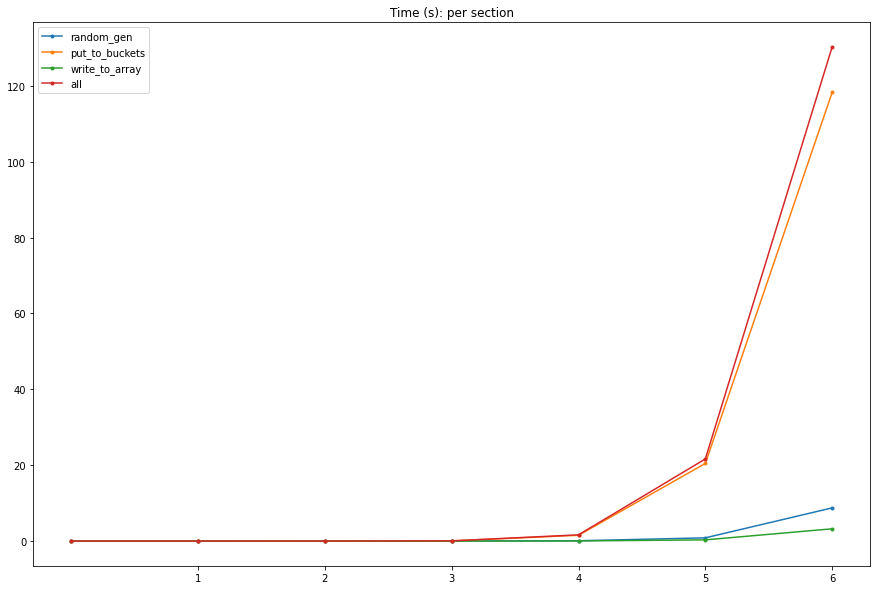
\includegraphics[width=17cm]{report2/images/Sequential/sam_time.png}
            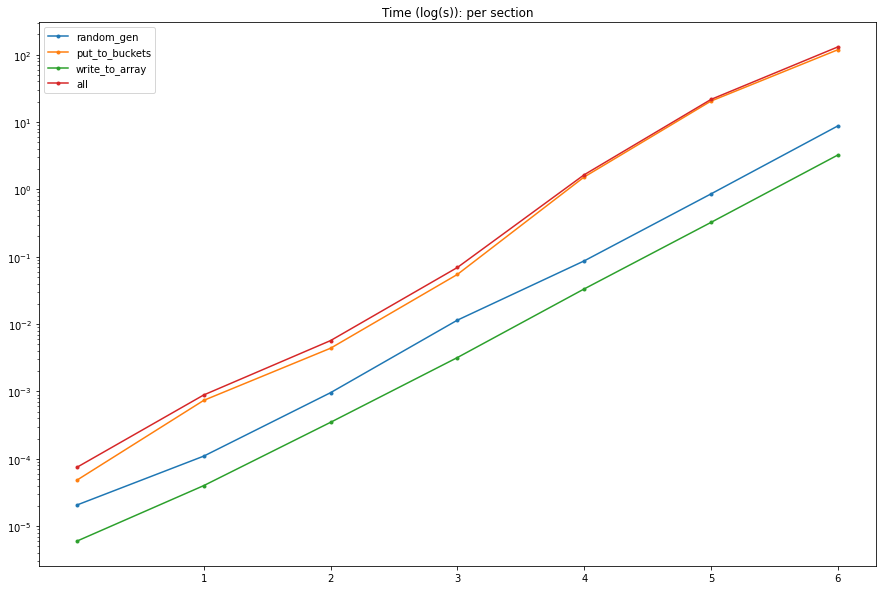
\includegraphics[width=17cm]{report2/images/Sequential/sam_time_log.png}
            \caption{Pomiar czasu wykonania programu, w wersji pierwszej, wykonywanego sekwencyjnie, w zależności od rozmiaru tablicy (od ${10^{3}}$ do ${10^{9}}$). }
        \end{figure}

        \begin{figure}[h!]
            \centering
            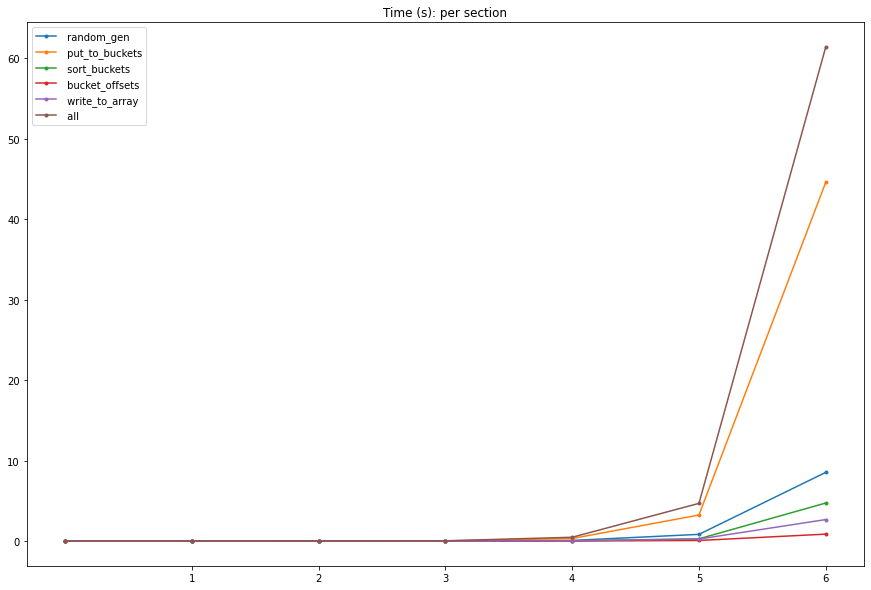
\includegraphics[width=17cm]{report2/images/Sequential/time.png}
            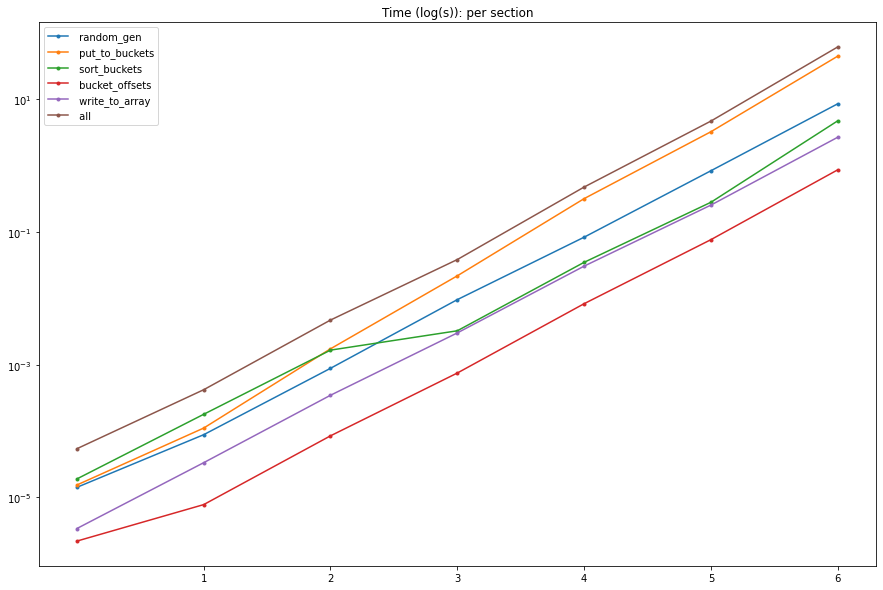
\includegraphics[width=17cm]{report2/images/Sequential/time_log.png}
            \caption{Pomiar czasu wykonania programu, w wersji drugiej, wykonywanego sekwencyjnie, w zależności od rozmiaru tablicy (od ${10^{3}}$ do ${10^{9}}$). }
        \end{figure}\\
    
    \FloatBarrier
    % \newline
    % \newpage
    
    \subsection{Badanie przyśpieszenia algorytmu}
        Analizując zmianę czasu wykonania programu w zależności od ilości rdzeni na których zrównoleglany był algorytm, zauważyć możemy że czas wykonania algorytmu w wersji pierwszej spada jednostajnie według oczekiwanej krzywej. W wersji drugiej, czas  wykonania zmienia się skokowo w nieoczekiwany sposób. Jest to zaskakujący wynik, którego nie oczekiwałem, dlatego uruchomiłem program w tej wersji także na komputerze wyposażonym w procesor \textit{Intel i7-8550u} z czterema rdzeniami roboczymi i ośmioma wątkami. W tym przypadku otrzymałem wyniki dużo bardziej zbliżone do oczekiwanych (z jedynym załamaniem wynikającym z hyperthreadingu), dlatego zaburzenia uznaję za spowodowane specyficzną architekturą procesora z którego początkowo korzystałem (architektura \textit{ARM}, rdzenie o różnej wydajności). 
        % \begin{figure}[h!]
        %     \centering
        %     \caption{Pomiar czasu wykonania programu, w wersji pierwszej, w zależności od ilości rdzeni, dla tablicy ${10^{9}}$. }
        % \end{figure}
        
        \begin{figure}[h!]
            \centering
            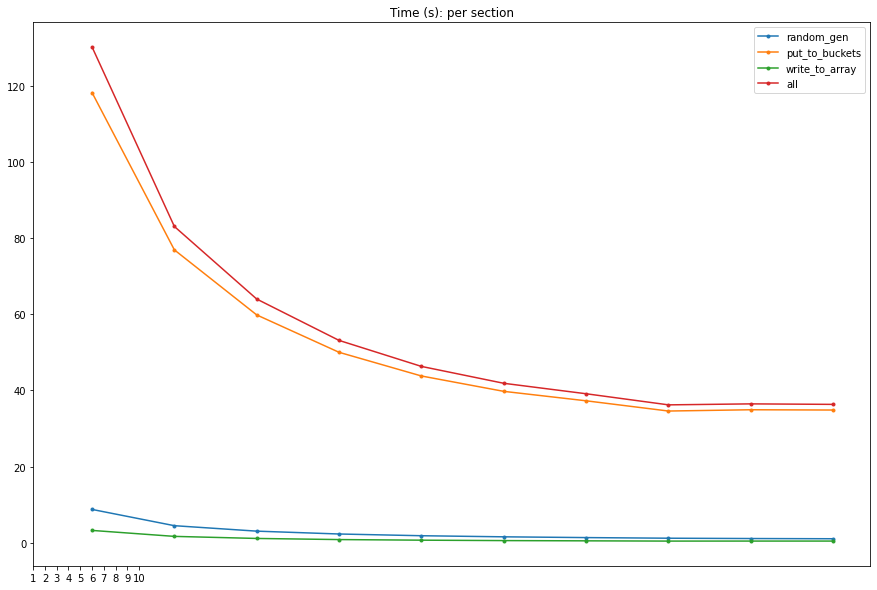
\includegraphics[width=17cm]{report2/images/Speedup/sam_time.png}
            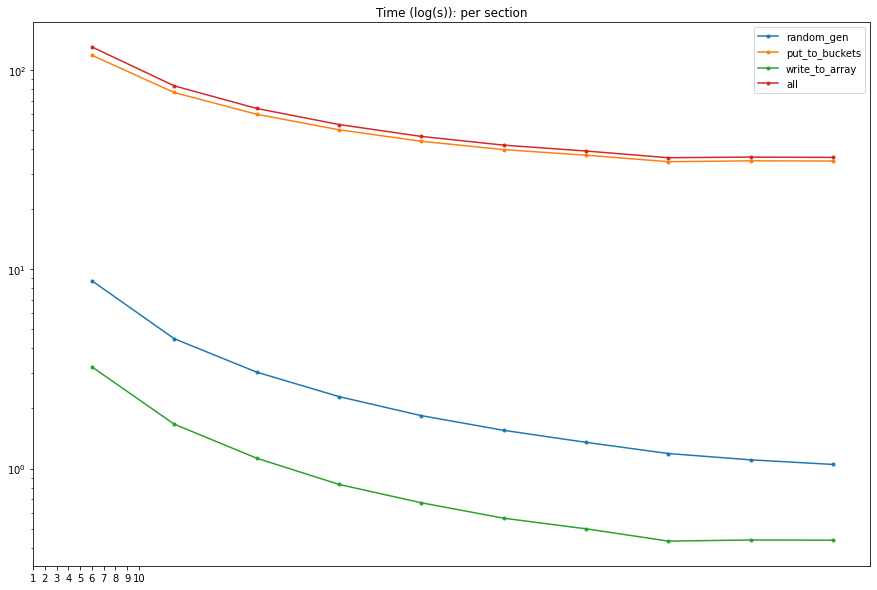
\includegraphics[width=17cm]{report2/images/Speedup/sam_time_log.png}
            \caption{Pomiar czasu wykonania programu, w wersji pierwszej, w zależności od ilości rdzeni, dla tablicy ${10^{9}}$. }
        \end{figure}

        \newpage
        \begin{figure}[h!]
            \centering
            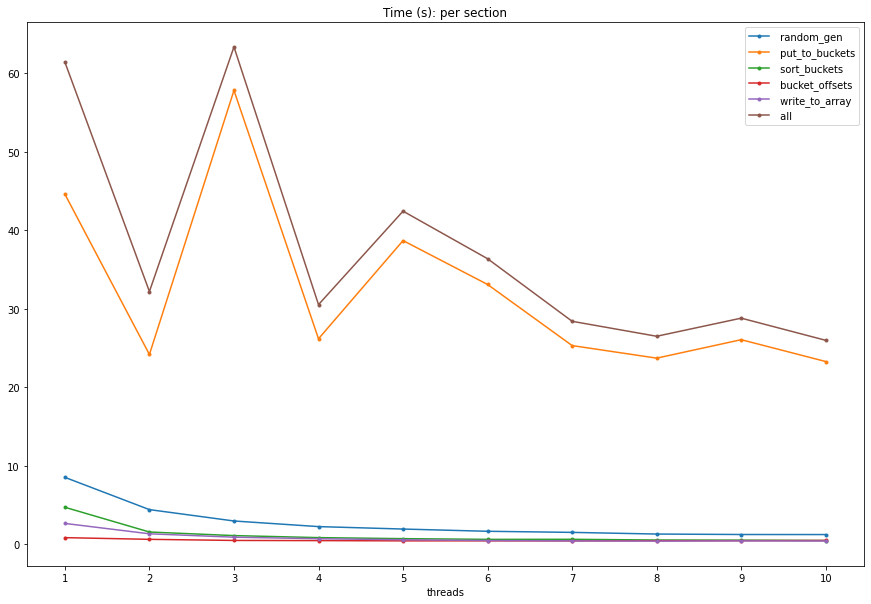
\includegraphics[width=17cm]{report2/images/Speedup/time.png}
            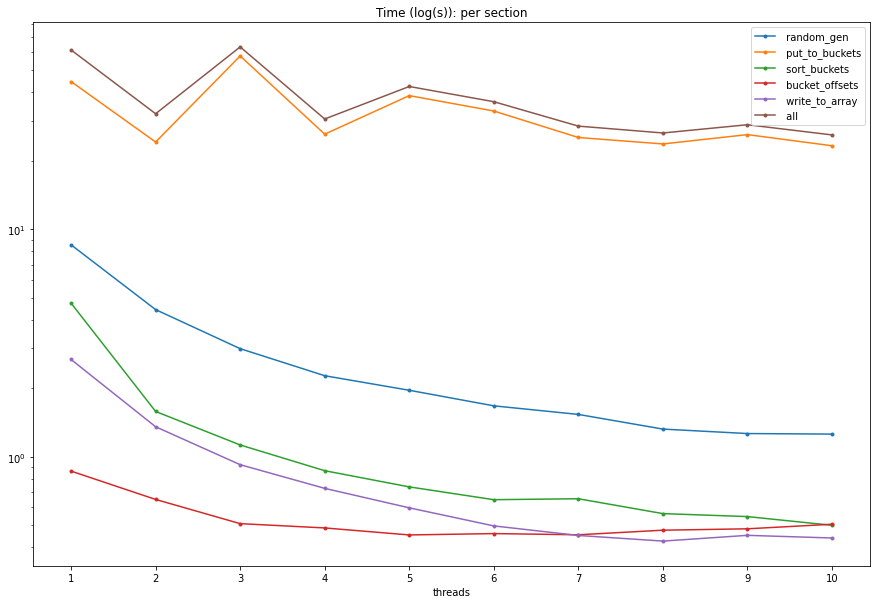
\includegraphics[width=17cm]{report2/images/Speedup/time_log.png}
            \caption{Pomiar czasu wykonania programu, w wersji drugiej, w zależności od ilości rdzeni, dla tablicy ${10^{9}}$. }
        \end{figure}
        
        \begin{figure}[h!]
            \centering
            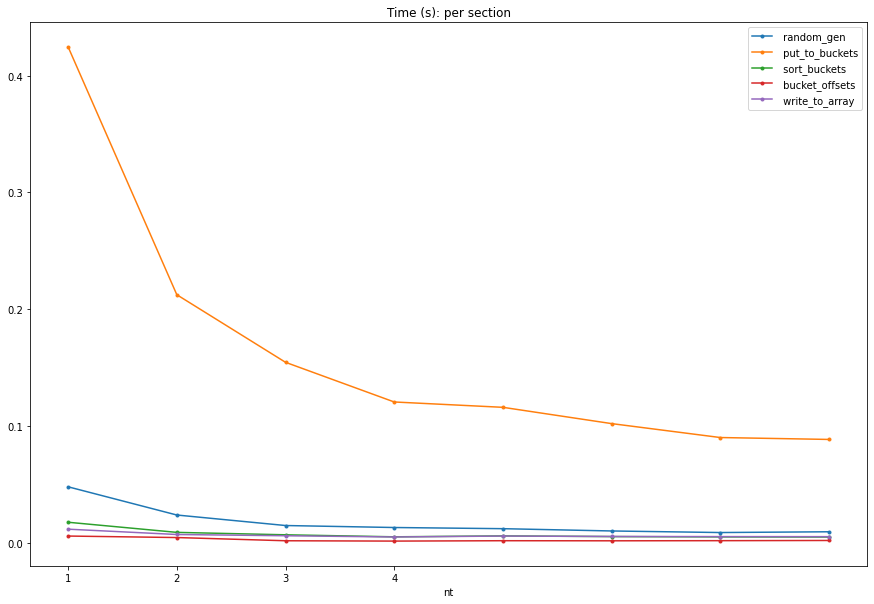
\includegraphics[width=17cm]{report2/images/Speedup/time_i7.png}
            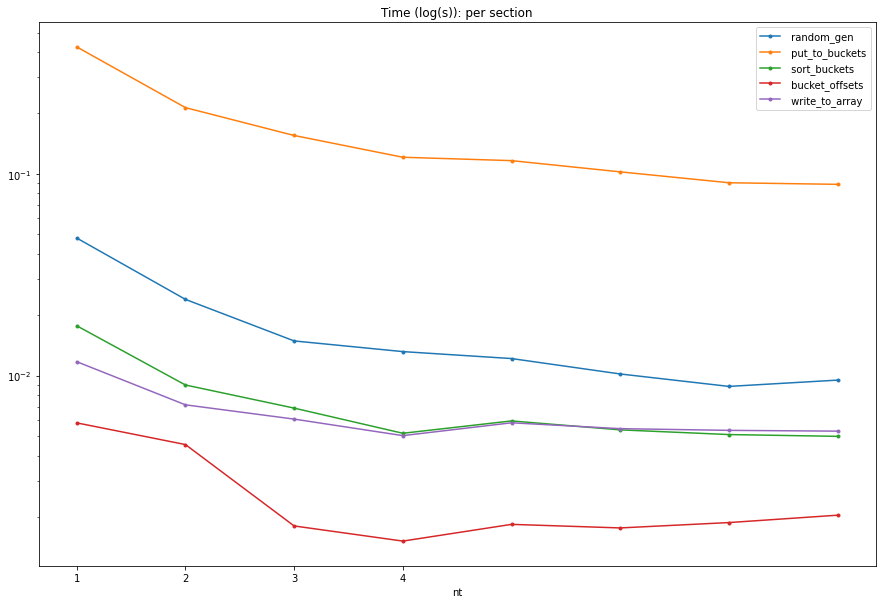
\includegraphics[width=17cm]{report2/images/Speedup/time_log_i7.png}
            \caption{Pomiar czasu wykonania programu, w wersji drugiej, w zależności od ilości rdzeni, dla tablicy ${10^{9}}$, uruchamianego na procesorze \textit{Intel i7}. }
        \end{figure}
    \FloatBarrier

        \newpage
        % Speedup
        Następnie przygotowałem pomiary przyśpieszenia algorytmu. We wszystkich przypadkach program przyśpieszał znacząco wraz ze wzrostem ilości rdzeni. W przypadku wersji pierwszej, ponownie wykres najbardziej przypominał oczekiwany. W przypadku wersji drugiej uruchomionej na procesorze \textit{i7} zauważyć możemy załamanie wynikające z \textit{hyperthreadingu} po wzroście powyżej czterech wątków. 
        \begin{figure}[h!]
            \centering
            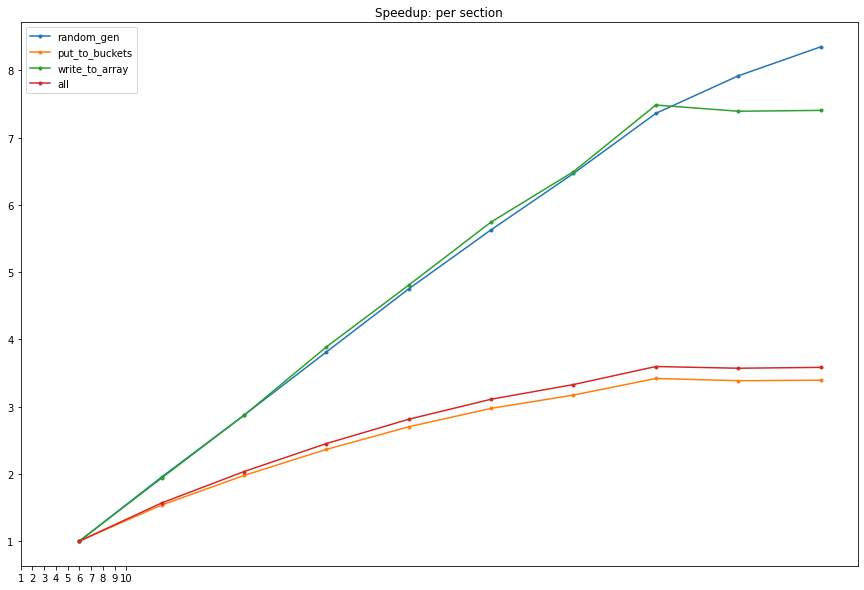
\includegraphics[width=17cm]{report2/images/Speedup/sam_speedup.png}        
            \caption{Pomiar przyśpieszenia programu, w wersji pierwszej, dla tablicy ${10^{9}}$. }
        \end{figure}
        
        \newpage
        \begin{figure}[h!]
            \centering
            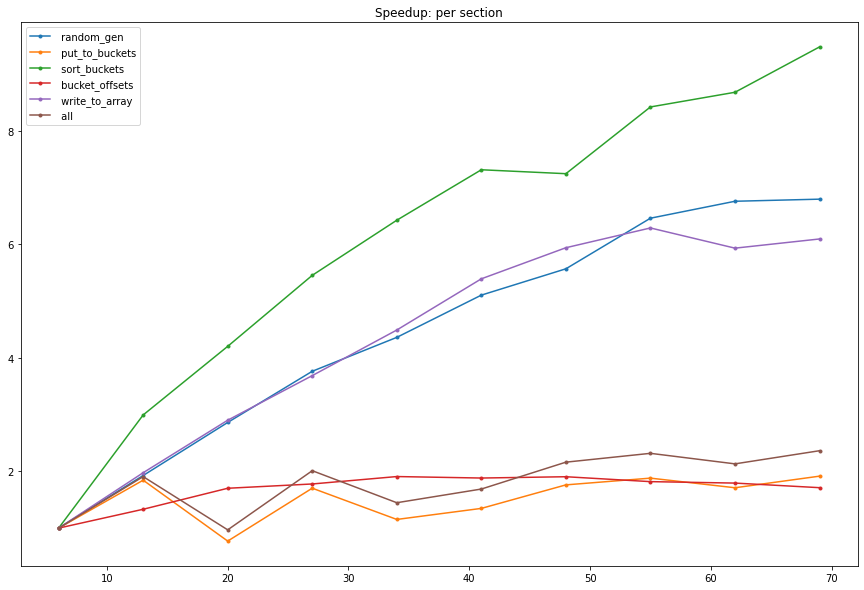
\includegraphics[width=15cm]{report2/images/Speedup/speedup.png}        
            \caption{Pomiar przyśpieszenia programu, w wersji drugiej, dla tablicy ${10^{9}}$. }
        \end{figure}
        
        \begin{figure}[h!]
            \centering
            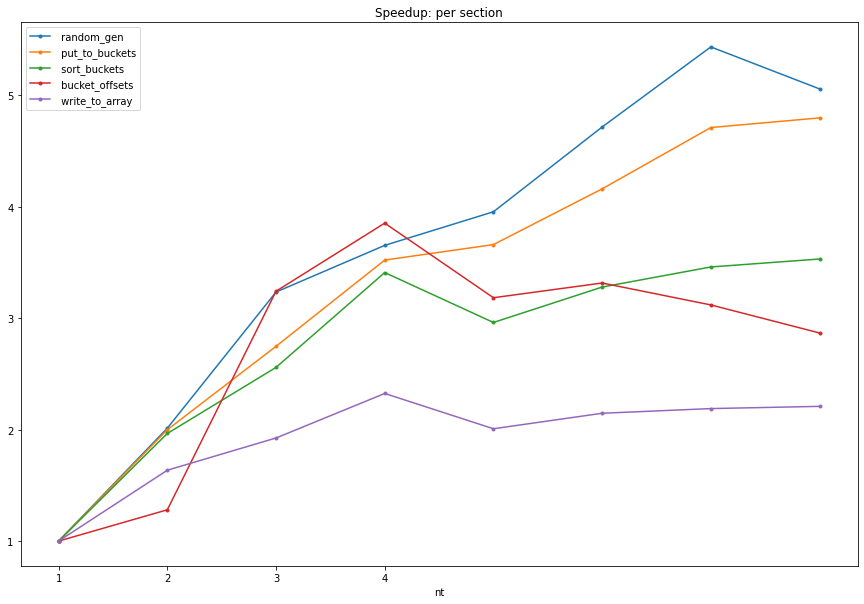
\includegraphics[width=15cm]{report2/images/Speedup/speedup_i7.png}        
            \caption{Pomiar przyśpieszenia programu, w wersji drugiej, dla tablicy ${10^{9}}$, uruchamianego na procesorze \textit{Intel i7}. }
        \end{figure}
    
    \newpage
    \subsection{Porównanie implementacji}
    W celu porównania złożoności obliczeniowej i czasu wykonania obu wersji algorytmu równoległego przygotowałem wykres czasu wykonania i przyśpieszenia dla stałego rozmiaru tablicy wejściowej (wynoszącego $1000 000 000$) w zależności od ilości rdzeni na których algorytm był zrównoleglany. Oba programy uruchamiane były na tym samym środowisku sprzętowym. Zaobserwować możemy dużo niższe czasy wykonania, niezależnie od ilości rdzeni na których program był uruchamiany, programu w wersji w której każdy z wątków czyta jedynie fragment tablicy wejściowej rozdzielając do kubełków. Przyśpieszenia procentowe są co do wartości mniejsze w wersji drugiej, co paradoksalnie może wynikać z mniejsze ilości obliczeń wykonywanych przez algorytm. 
    
        \begin{figure}[h!]
            \centering
            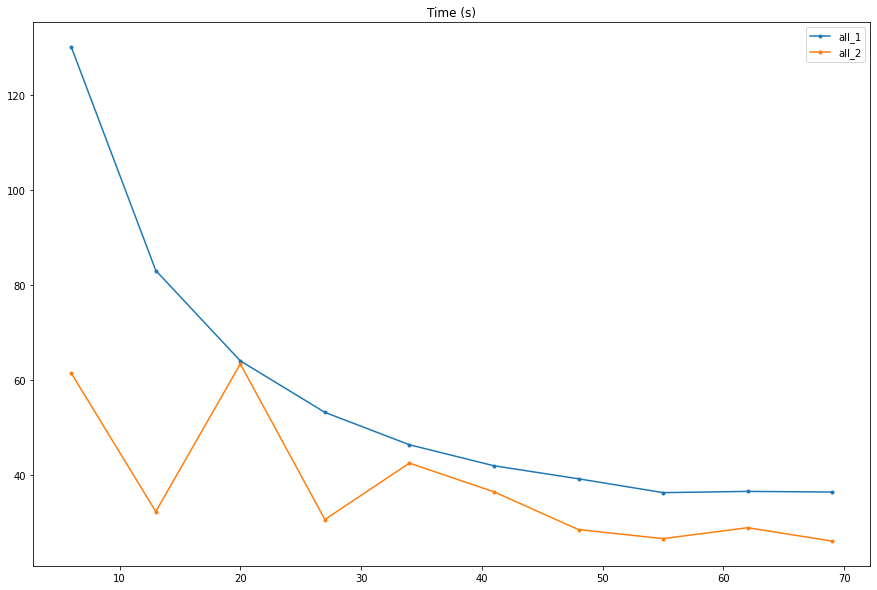
\includegraphics[width=17cm]{report2/images/Compare/time.png}
            \caption{Pomiar czasu wykonania programu, w zależności od wersji i ilości rdzeni. }
        \end{figure}
    
    \newpage    
        \begin{figure}[h!]
            \centering
            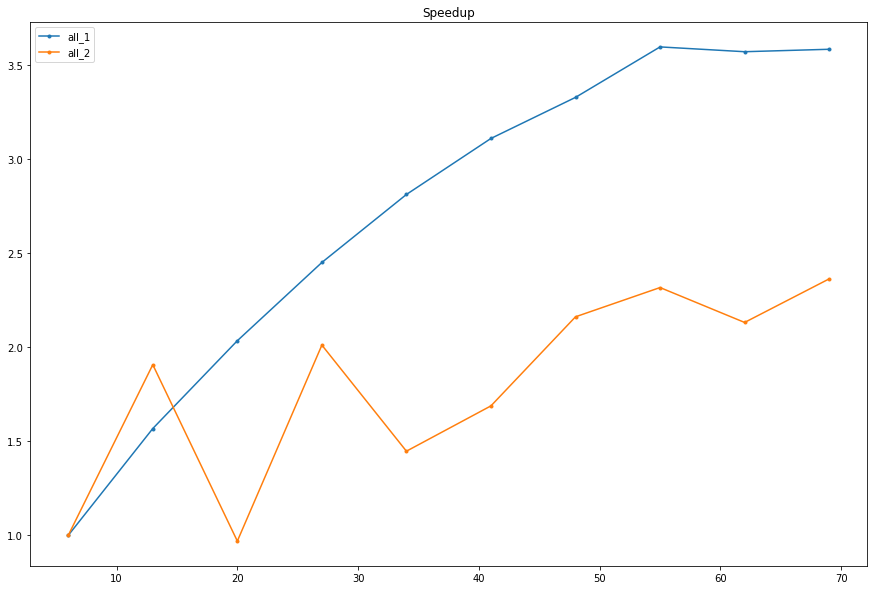
\includegraphics[width=17cm]{report2/images/Compare/speedup.png}
            \caption{Pomiar przyśpieszenia, w zależności od wersji i ilości rdzeni.}
        \end{figure}
        
    \FloatBarrier
    \newpage
    \subsection{Kod programu (wersja druga)}
        \lstinputlisting[language=c]{../lab3/main.c}

\end{document}
